\documentclass[12pt]{article}

\usepackage{booktabs}
\usepackage{graphicx}
\usepackage{subcaption}
\usepackage{amsmath}
\usepackage{setspace}
\usepackage[margin=1in]{geometry}
\usepackage[hidelinks]{hyperref}

\widowpenalty10000
\clubpenalty10000

\graphicspath{{../../output/}}

\title{How Much Are People Using Claude for Election Information?\thanks{Claude Fable 5 (Anthropic) wrote the analysis code and most of this memo. I reviewed the code and text after the fact and checked them for accuracy.}}
\author{Daniel M. Thompson}
\date{\today}

\begin{document}

\maketitle

\onehalfspacing

\section*{Estimating the Effect of Primary Elections on the Rate of Political Claude Conversations}

We want to know whether people use AI assistants to research upcoming elections. Individual AI conversations are private and usage data are proprietary, but the Anthropic Economic Index (AEI) now publishes anonymized, aggregated Claude usage at a useful resolution: the share of each U.S. state's conversations assigned to each topic in a hierarchy, by calendar month, for April and May 2026.\footnote{Released CC-BY at \url{https://huggingface.co/datasets/Anthropic/EconomicIndex}, \texttt{release\_2026\_06\_26}. Cells with too few conversations to protect privacy are not published, and topic taxonomies are re-estimated in each release, so we use only this release.} Our outcome is the share of a state's conversations in the ``Politics and public record'' topic, the broadest political category, published in both months for 33 states.

The 2026 primary calendar supplies the variation: statewide primaries were spread from March through September, so residents of different states needed election information in different months. Eight states in the panel held their primaries in May (Alabama, Georgia, Idaho, Indiana, Louisiana, Ohio, Oregon, Pennsylvania); 22 states held theirs between June and September and serve as controls. Texas, North Carolina, and Illinois held March primaries and are excluded as already treated. We estimate a difference-in-differences,
\begin{equation}
y_{sm} = \delta \left(\text{May primary}_s \times \text{May}_m\right) + \alpha_s + \gamma_m + \varepsilon_{sm},
\end{equation}
where $y_{sm}$ is the politics-topic share in state $s$ and month $m \in \{\text{April}, \text{May}\}$, with state and month fixed effects and standard errors clustered by state. The identifying assumption is that, absent a primary, May-primary states' conversation topics would have moved like later-primary states'.

\section*{Claude Conversations Shift Toward Politics When a State Holds Its Primary}

Holding a primary shifts a state's Claude conversations toward politics. In April, before any of them voted, the eight May-primary states devoted 0.40 percent of conversations to the politics topic; in May, their primary month, 0.50 percent. The 22 later-primary states sat at 0.48 percent in both months (Figure~\ref{fig:did}a). The shift is broad-based rather than driven by an outlier: seven of the eight treated states move up, with a median change of $+$0.10 percentage points, while control-state changes straddle zero (Figure~\ref{fig:did}b).

Table~\ref{tab:aei_did} reports the estimates. The primary raises the politics-topic share by 0.10 percentage points (s.e.\ 0.04)---22 percent of the control-group May mean---and the estimate is similar when June-primary states, where mail voting begins in May, are dropped from the control group (0.09), and in logs (a 27 percent increase, s.e.\ 9 percent). With 30 states, the design can detect effects of about 0.11 percentage points, so the estimate sits at the edge of detectability: we can rule out effects twice as large but not half as large.

One corroborating pattern: the AEI's narrow ``Elections'' subtopic is published only where conversation counts clear the privacy floor. It appears in three states in April but eight in May, and the newly published states are disproportionately May-primary states (Oregon, Pennsylvania, Georgia)---election conversations became common enough to publish exactly where and when primaries occurred.

\begin{figure}[p]
\centering
\begin{subfigure}{0.85\textwidth}
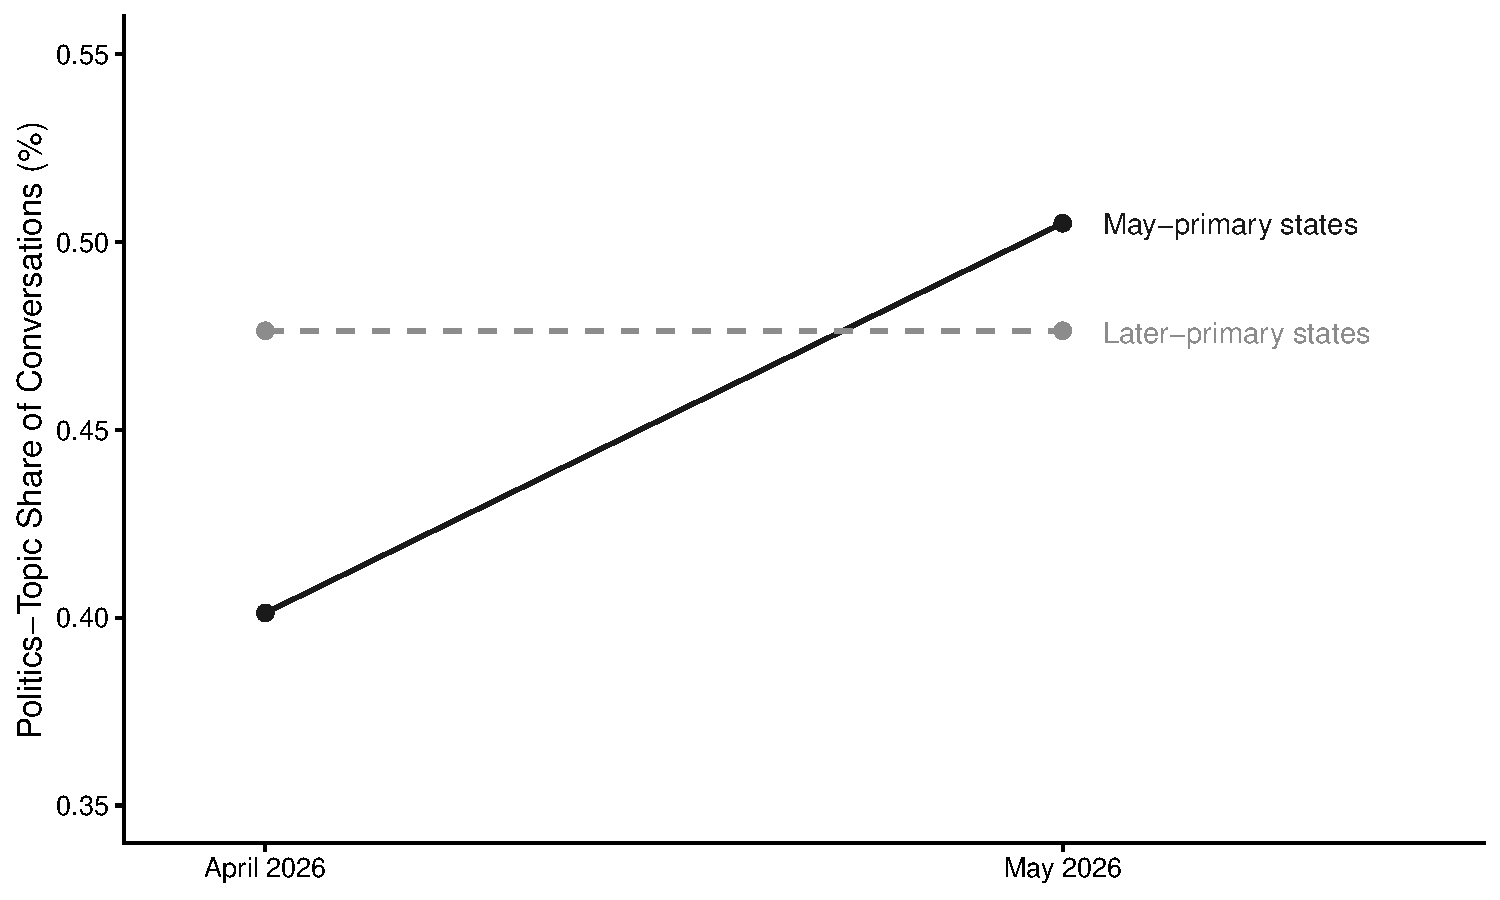
\includegraphics[width=\textwidth]{aei_politics_did.pdf}
\caption{Group means}
\end{subfigure}
\begin{subfigure}{0.85\textwidth}
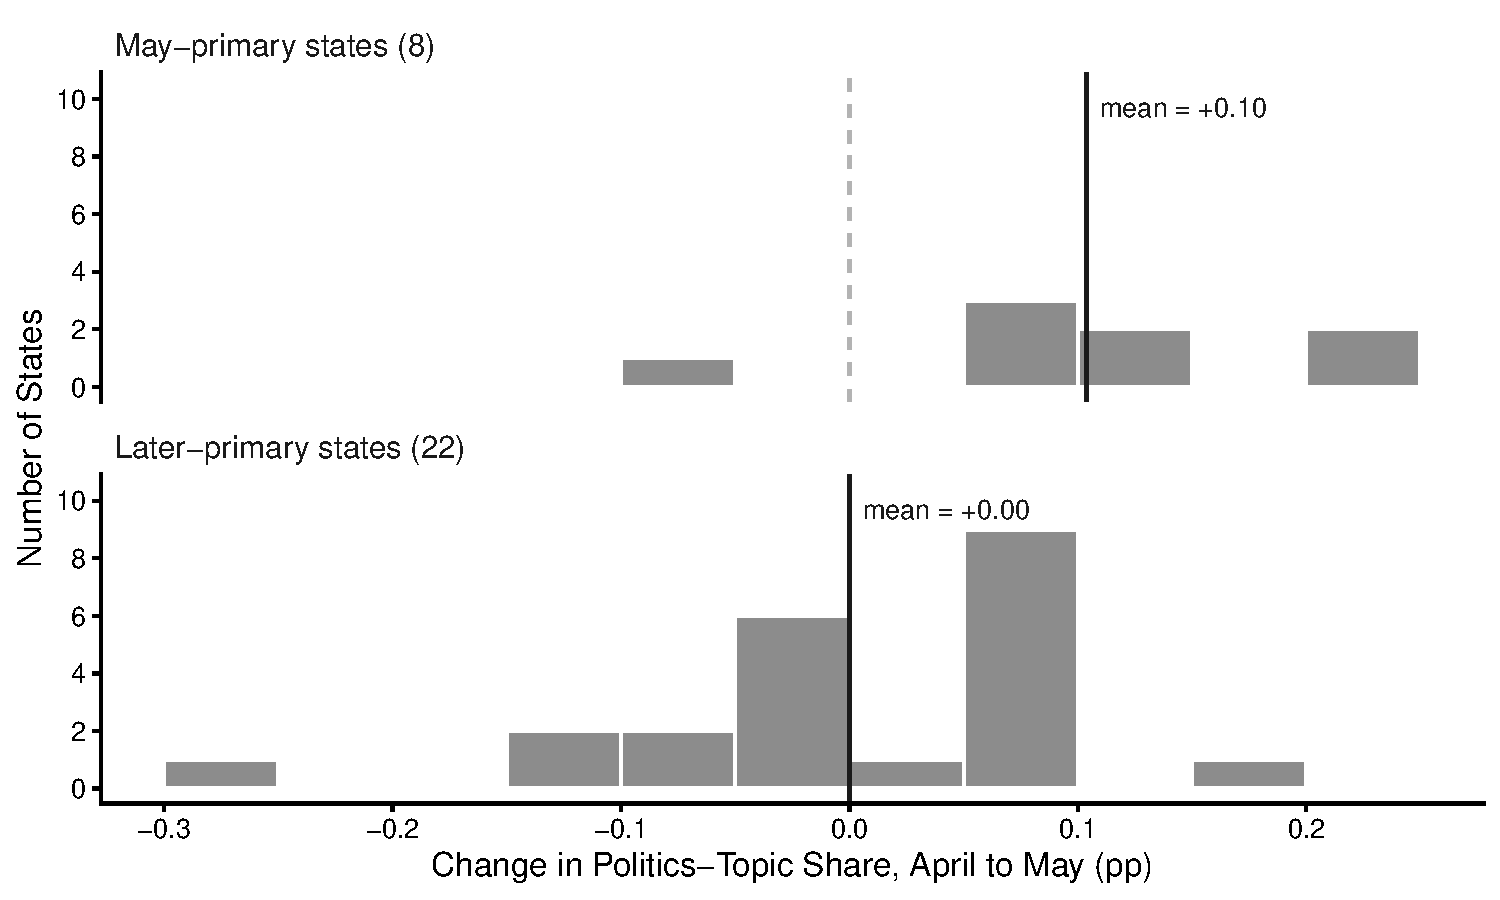
\includegraphics[width=\textwidth]{aei_change_hist.pdf}
\caption{Distribution of state-level changes}
\end{subfigure}
\caption{\textbf{The politics-topic share of Claude conversations rises when a state holds its primary.} Panel (a) plots the mean politics-topic share of conversations in April and May 2026 for the eight states with May 2026 primaries and the 22 states with June-September primaries; March-primary states are excluded. Panel (b) shows each state's April-to-May change, by group, with vertical lines at the group means.}
\label{fig:did}
\end{figure}

\begin{table}[t]
\centering
\caption{\textbf{Claude Conversations Shift Toward Politics When a State Holds Its Primary.}\label{tab:aei_did}}
\begin{tabular}{lccc}
\toprule \toprule
 & \multicolumn{2}{c}{Politics-Topic Share (\%)} & Log Share \\
\cmidrule(lr){2-3} \cmidrule(lr){4-4}
 & (1) & (2) & (3) \\
\midrule
Primary $\times$ May & 0.10 & 0.09 & 0.24 \\
 & (0.04) & (0.04) & (0.09) \\[2mm]
\# States & 30 & 20 & 30 \\
\# Treated States & 8 & 8 & 8 \\
\# Observations & 60 & 40 & 60 \\
Control May Mean & 0.48 & 0.45 & 0.48 \\
Minimum Detectable Effect & 0.11 & 0.12 & 0.24 \\
\midrule
State Fixed Effects & Yes & Yes & Yes \\
Month Fixed Effects & Yes & Yes & Yes \\
Excl.\ June-Primary Controls & No & Yes & No \\
\bottomrule \bottomrule
\multicolumn{4}{p{0.95\textwidth}}{\footnotesize \textit{Notes}: Each column reports a difference-in-differences estimate comparing the politics-topic share of Claude conversations in April and May 2026 between states holding a statewide primary in May 2026 and states with later primaries. The outcome in columns 1 and 2 is the percent of a state's conversations assigned to the ``Politics and public record'' topic in the Anthropic Economic Index; column 3 uses its natural log. Texas, North Carolina, and Illinois, which held March primaries, are excluded. Column 2 further drops control states with June primaries, whose mail voting begins in May. Standard errors clustered by state are in parentheses. The minimum detectable effect is 2.80 times the standard error.} \\
\end{tabular}
\end{table}


\section*{What These Estimates Can and Cannot Tell Us}

Four limitations to keep in mind. First, the panel is two months long, so the design is a single pre/post contrast across primary cohorts; we cannot examine pre-trends the way a longer panel would allow. Second, the privacy threshold limits the sample to 30 larger states and rules out the narrow ``Elections'' topic as an outcome; the ``Politics and public record'' topic includes political conversation beyond election logistics. Third, values are published rounded to two decimals, which adds noise that is meaningful relative to a 0.10-point effect. Fourth, the estimates describe the volume of politics-related conversations, not their content or accuracy.

\end{document}
